\section{Resultados}

\subsection{Perfil promedio del evento}

La Figura~\ref{fig:event} muestra la trayectoria promedio relativa al periodo pre-evento. Visualmente, el patron es heterogeneo: hay eventos con aumentos y eventos con caidas de inflacion post-ajuste.

\begin{figure}[H]
\centering
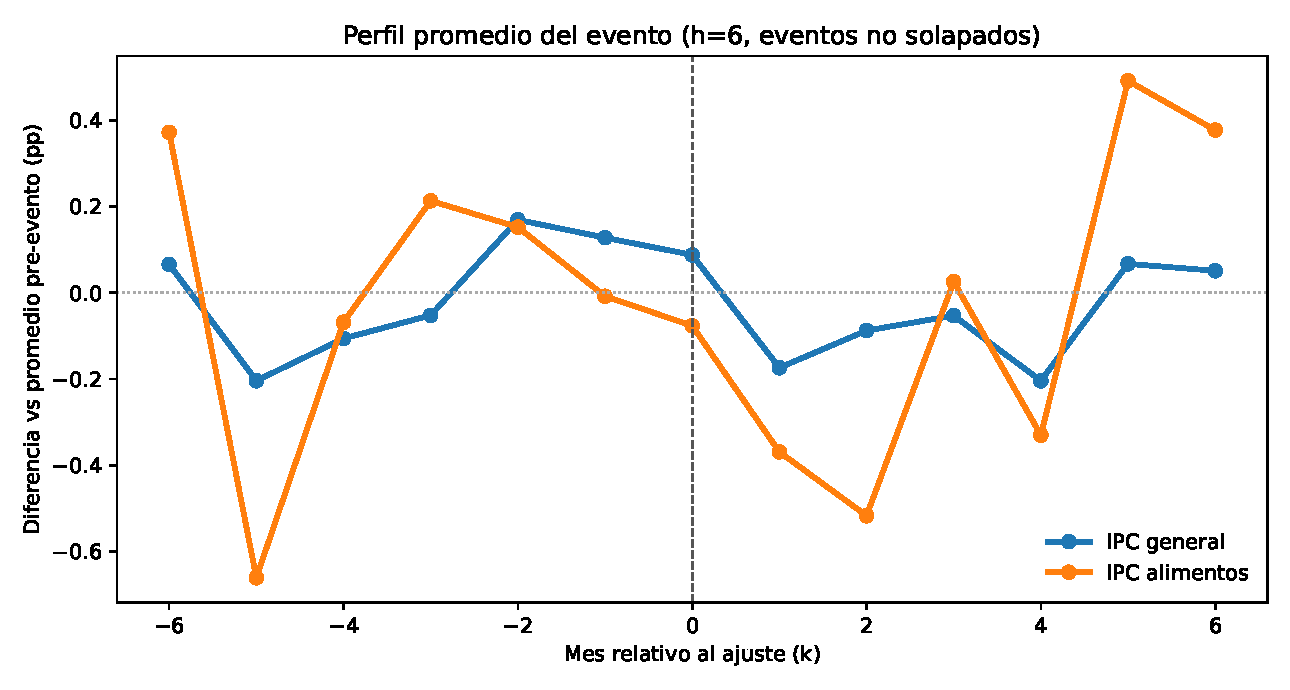
\includegraphics[width=0.92\textwidth]{figures/fig_event_profile.pdf}
\caption{Perfil promedio de inflacion alrededor del ajuste del SML (h=6, eventos no solapados)}
\label{fig:event}
\end{figure}

A nivel promedio, el EI en IPC general es \eiGeneralMain{} pp y en IPC alimentos \eiAlimentosMain{} pp.

\subsection{Evidencia placebo}

La Figura~\ref{fig:placebo} ubica el EI observado frente a su distribucion placebo. Los p-valores de referencia son \pGeneralMain{} para IPC general y \pAlimentosMain{} para IPC alimentos. Esto sugiere cautela frente a inferencias fuertes de causalidad en la especificacion principal.

\begin{figure}[H]
\centering
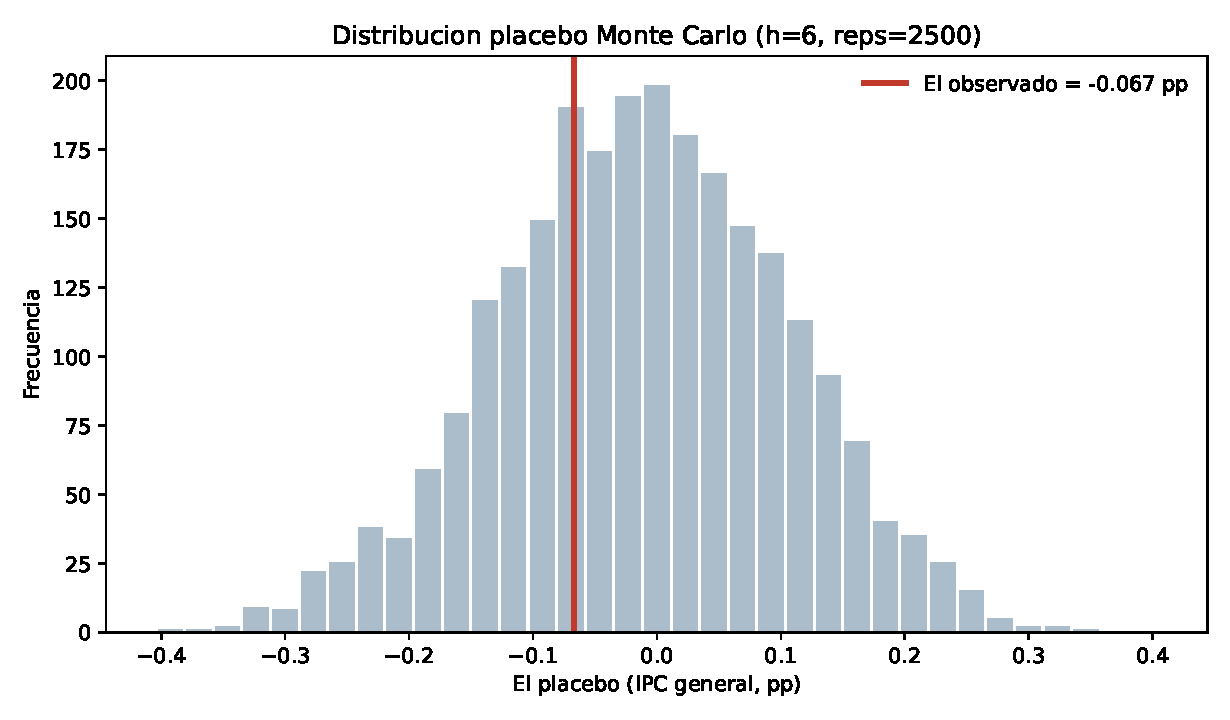
\includegraphics[width=0.85\textwidth]{figures/fig_placebo_hist.pdf}
\caption{Distribucion placebo Monte Carlo para EI de IPC general}
\label{fig:placebo}
\end{figure}

\subsection{Robustez de ventanas y limpieza de solapamiento}

La Tabla~\ref{tab:rob} resume sensibilidad por horizonte ($h=3,6,9$) y criterio de solapamiento. La magnitud y significancia descriptiva varian con la especificacion, consistente con shocks macro y composicion temporal de eventos.

\begin{table}[H]
\centering
\caption{Robustez por horizonte y criterio de solapamiento}
\label{tab:rob}
\begin{tabular}{rlrrrrr}
\toprule
h & Solap. & N & EI gen & EI alim & p gen & p alim\\
\midrule
3 & all & 24 & -0.269 & -0.500 & 0.095 & 0.178\\
3 & clean & 24 & -0.269 & -0.500 & 0.095 & 0.178\\
6 & all & 23 & -0.149 & -0.184 & 0.194 & 0.456\\
6 & clean & 22 & -0.067 & -0.054 & 0.579 & 0.821\\
9 & all & 22 & -0.042 & 0.036 & 0.613 & 0.842\\
9 & clean & 18 & 0.069 & 0.246 & 0.481 & 0.189\\
\bottomrule
\end{tabular}

\end{table}

\subsection{Contexto laboral y de hogares}

La Figura~\ref{fig:contexto} integra series trimestrales de R02 y R01 con marcas de trimestres de ajuste del SML. Esta lectura permite contextualizar el fenomeno en dinamicas de formalidad, conectividad y condiciones del hogar.

\begin{figure}[H]
\centering
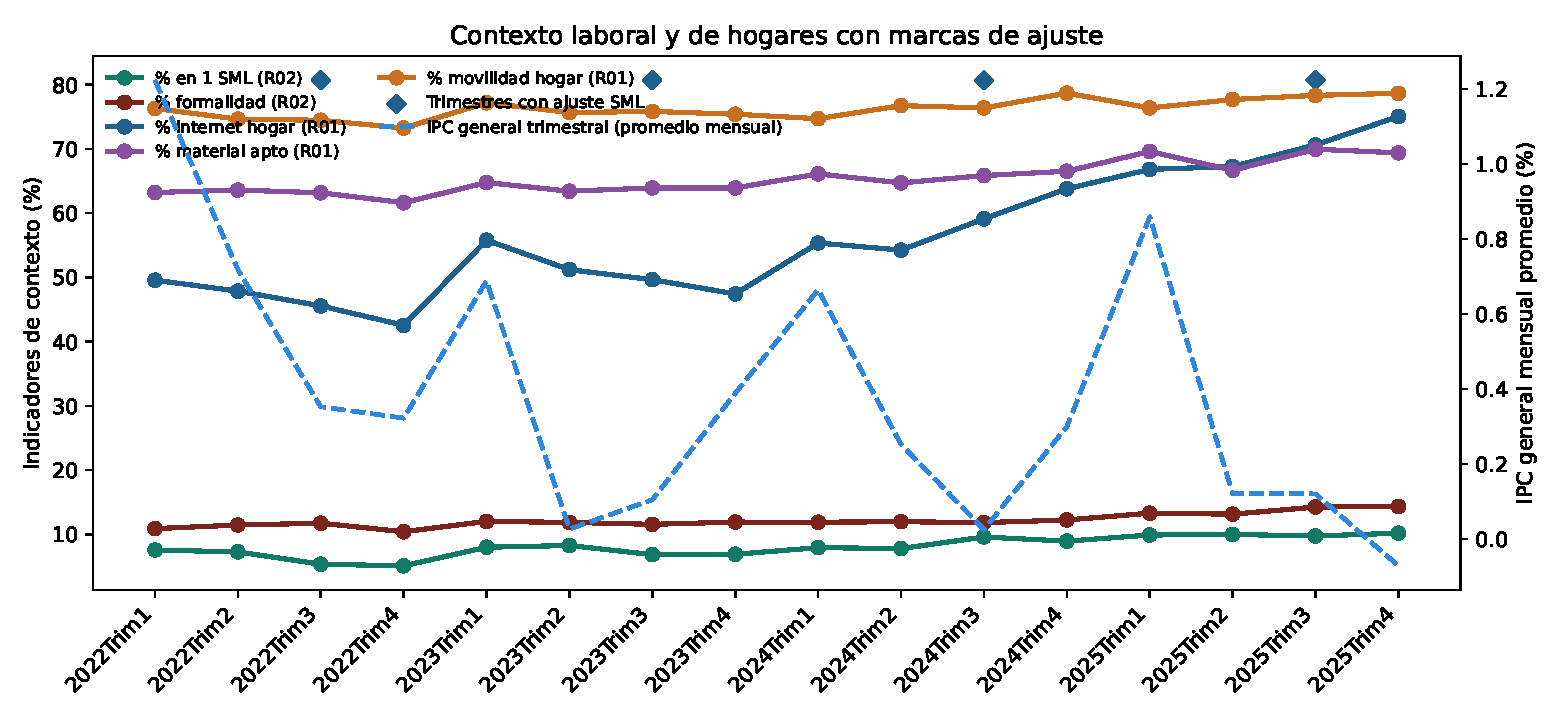
\includegraphics[width=0.98\textwidth]{figures/fig_contexto_trimestral.pdf}
\caption{Contexto R02 + R01 con marcas de trimestres de ajuste del SML}
\label{fig:contexto}
\end{figure}

Como complemento distributivo, la Figura~\ref{fig:densidad} muestra concentracion de masa alrededor de 1 SML (banda $\pm 10\%$), en linea con patrones de bunching descriptivo.

\begin{figure}[H]
\centering
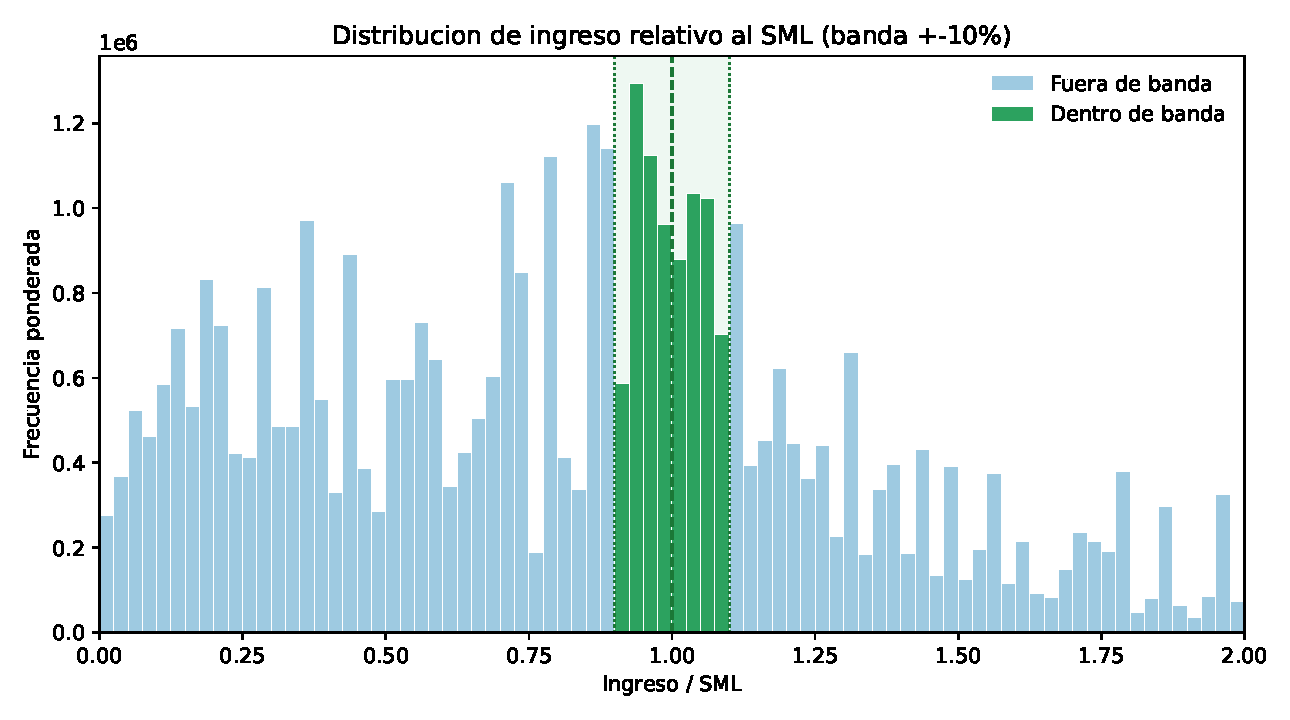
\includegraphics[width=0.86\textwidth]{figures/fig_density_rel_sml.pdf}
\caption{Distribucion de ingreso relativo al SML y banda $\pm 10\%$}
\label{fig:densidad}
\end{figure}

\subsection{Auditoria por evento}

Para trazabilidad, la Tabla~\ref{tab:eventos} reporta ajuste, EI y coeficientes de traspaso por evento individual.

\begin{table}[H]
\centering
\caption{Metricas por evento (especificacion principal)}
\label{tab:eventos}
\begin{tabular}{lrrrrr}
\toprule
Fecha & Ajuste (pp) & EI IPC gen & EI IPC alim & CT gen & CT alim\\
\midrule
1996-04-01 & 10.000 & -0.865 & -1.002 & -0.087 & -0.100\\
1997-01-01 & 10.000 & 0.509 & 0.716 & 0.051 & 0.072\\
1998-03-01 & 12.000 & 0.514 & 0.641 & 0.043 & 0.053\\
2000-02-01 & 15.000 & 0.026 & -0.365 & 0.002 & -0.024\\
2001-05-01 & 15.000 & -0.340 & -1.295 & -0.023 & -0.086\\
2002-08-01 & 12.000 & 0.621 & 2.072 & 0.052 & 0.173\\
2005-04-01 & 12.000 & 0.262 & 0.220 & 0.022 & 0.018\\
2006-04-01 & 12.000 & -0.672 & -1.513 & -0.056 & -0.126\\
2007-10-01 & 10.000 & -0.347 & -1.139 & -0.035 & -0.114\\
2009-05-01 & 5.000 & 0.385 & 1.334 & 0.077 & 0.267\\
2010-07-01 & 7.000 & 0.660 & 1.702 & 0.094 & 0.243\\
2011-04-01 & 10.000 & -1.480 & -3.870 & -0.148 & -0.387\\
2014-03-01 & 10.000 & -0.663 & -1.486 & -0.066 & -0.149\\
2016-12-01 & 7.700 & 0.239 & 0.413 & 0.031 & 0.054\\
2017-07-01 & 3.900 & 0.193 & 0.615 & 0.050 & 0.158\\
2018-07-01 & 3.500 & -0.053 & 0.374 & -0.015 & 0.107\\
2019-07-01 & 3.800 & -0.035 & 0.246 & -0.009 & 0.065\\
2021-07-01 & 4.400 & 0.664 & 1.848 & 0.151 & 0.420\\
2022-07-01 & 11.400 & -0.556 & -0.418 & -0.049 & -0.037\\
2023-07-01 & 5.100 & 0.043 & 0.589 & 0.008 & 0.116\\
2024-07-01 & 4.400 & -0.148 & -0.466 & -0.034 & -0.106\\
2025-07-01 & 3.600 & -0.430 & -0.398 & -0.119 & -0.111\\
\bottomrule
\end{tabular}

\end{table}

\begin{table}[H]
\centering
\caption{Contexto trimestral 2025 (R02 + R01)}
\label{tab:ctx2025}
\begin{tabular}{lrrrrr}
\toprule
Trimestre & \% 1 SML & \% formalidad & \% internet & \% material apto & \% movilidad\\
\midrule
2025Trim1 & 9.904 & 13.304 & 66.805 & 69.593 & 76.374\\
2025Trim2 & 9.994 & 13.146 & 67.259 & 66.671 & 77.682\\
2025Trim3 & 9.748 & 14.252 & 70.629 & 69.951 & 78.332\\
2025Trim4 & 10.193 & 14.357 & 75.042 & 69.378 & 78.649\\
\bottomrule
\end{tabular}

\end{table}
